\documentclass[10pt, conference, compsocconf]{IEEEtran}

% packages
\usepackage{algorithm}
\usepackage{algorithmic}
\usepackage{amsfonts} % for R symbol (the set of real numbers)
\usepackage{color}
\usepackage[pdftex]{graphicx}
\usepackage{hyperref}
\usepackage{mathtools}
\usepackage{multirow}
\usepackage{stmaryrd} % for llbracket and rrbracket
\DeclarePairedDelimiter{\ceil}{\lceil}{\rceil}
\DeclarePairedDelimiter{\floor}{\lfloor}{\rfloor}

% new commands
\newcommand{\todo}[1]{\marginpar{\parbox{18mm}{\flushleft\tiny\color{red}\textbf{TODO}:
      #1}}}

\newcommand{\note}[1]{
  \color{blue}\emph{[Note: #1]}
  \color{black}
}


\begin{document}

\title{Sequential algorithms to split and merge ultra-high resolution 3D images}

\author{Final ordering
  to be discussed when the paper: Yongping/Val\'erie,
  Yuhong Yan, Tristan.\\
  Department of Computer Science and Software Engineering, Concordia University, Montreal, Quebec, Canada
}

\maketitle

\begin{abstract}
  \todo{The abstract goes here. DO NOT USE SPECIAL CHARACTERS,
    SYMBOLS, OR MATH IN YOUR TITLE OR ABSTRACT.} 
\end{abstract}


\section{Introduction}

Three-dimensional images that exceed typical memory size are
increasingly found in a variety of disciplines. BigBrain, for
instance, is a 3D histological image of the human brain that
represents 1~TB of data organized in 3600 planes at full resolution
(1$\mu$m in-plane), and 76~GB at a 40$\mu$m isotropic resolution
commonly used in neurosciences~\cite{amunts2013bigbrain}. Other
examples found in medical imaging, our primary domain of interest,
include \todo{electromicroscopy,spectroscopy-francoise-peyrin}. As
such images would typically be processed on a computing cluster,
possibly using locality-aware file systems such as HDFS, software
libraries are needed to split and merge such images efficiently. We
introduce and compare a family of algorithms to address this problem
in a sequential environment made of a single storage disk. We are
aware of the need for parallel algorithms that would split and merge
images to and from an array of disks but we plan to describe such
algorithms in a subsequent paper based on the results of the present
one. \todo{
There is BigBrain-1 rescanned at 1 micron in the plane. So resolution
is 1x1x20, 7404 slices. If raw data are about 1Tb, then multiply by
100 for an estimation of the size of the new image. }


%also in
%MB/s).

Images are split into chunks representing 3D blocks or 2D slices. We
assume that a block or slice fits in memory. The BigBrain would
perhaps be split into 125 chunks of 600~MB. The decision to split an
image into slices or blocks, and the size of the resulting chunks, may
be constrained by the application. Some applications, for instance
spatial filtering, would commonly require blocks while other ones such
as acquisition artifact removal would rather work on
slices. Flexibility is thus required in the splitting
scheme. Applications processing voxels individually, for instance
histogram computation or k-means clustering, could work on either
slices or blocks.

The main problem encountered in the context of this paper is the fact
that, if not ordered properly, data reads and writes might result in
extensive seek times that, as we illustrate below, drastically limit
the I/O performance. This problem is obviously related to the ordering
of data bytes in image files, which we assume is arbitrary but known
to the algorithm. The problem is also related to the geometry of the
chunks to extract or merge, which we again assume arbitrary but known
to the algorithm. In a nutshell, we are looking for algorithms to
reduce seek times while allowing for arbitrary chunk geometries and
arbitrary byte orders in data files. The main idea of the variations
presented in the remainder of the paper is to convert data orderings
in memory before writing them on disk. 

The literature looks remarkably scarce on the problem described
above. Parallel processing of 3D images has obviously been extensively
studied, but methods have focused more on geometrical approaches to
partition images and on load-balancing and task scheduling techniques
while we aim at algorithms to efficiently split or merge images
regardless of the geometry of the chunks \todo{do a serious literature
review on this topic}. Perhaps this lack of related works could be
attributed to the fact that disk I/O weren't a bottleneck until image
resolution reached a certain threshold. A relevant reference is the
description of the Open Connectome Data Cluster~\cite{burns2013open},
a data warehouse system that allows users to retrieve specific chunks
of large datasets. In this work, the problem of long seek times is
addressed by designing a specific file format based on space-filling
curves, that elegantly preserves spatial proximity on disk. However,
addressing the problem using a specific data organization optimizes
the system for specific chunk geometries, volumetric in this case,
while we aim at algorithms that support multiple types of geometries.

This paper makes the following contributions:
\begin{itemize}
  \item We propose a set of algorithms to split and merge 3D images
    that do not fit in memory.
  \item We model the performance (execution time) of these algorithms,
    based on a simple but realistic disk I/O model.
  \item We evaluate our model and algorithms on a representative
    use-case involving a 1~TB image a hard drive and a solid-state
    drive.
  \item We compare the algorithms in a variety of conditions based on the validated model.
\end{itemize}
Section~\ref{sec:algos} presents our algorithms and their complexity,
Section~\ref{sec:results} details the results and
Sections~\ref{sec:discussion} discusses them.

%\href{http://dl.acm.org/citation.cfm?id=218395}

\newpage

\section{Algorithms}
\label{sec:algos}

\todo{Overlapping blocks. non-cubic blocks.}

In our context, split and merge relate to the same dual
problem \todo{not so sure about this actually}. Without loss of
generality, we focus here on merging for the sake of concision. Our
goal then is to merge a set of $n$ chunks into a single reconstructed
3D image with $R$ voxels of size $b$. We assume that all chunks are of
identical size and that slices are squares and blocks are cubes.

Without loss of generality, we consider a file format where voxels are
written after alphanumerical sorting of their (x,y,z)
representation. That is, x slices are written one after the other, and
in every x slice, y rows are written one after the other. NIfTI, the
file format defined by the Neuroimaging Informatics Technology
Initiative NIfTI\footnote{\url{https://nifti.nimh.nih.gov}} is such a
format, used by the vast majority of the neuroimaging community. In
the remainder, we use the term ``slice" for ``x slice".

\subsection{Notations}

We adopt the following notations:
\begin{itemize}
\item $R=D^3$: number of voxels in the reconstructed image.
\item $b$: number of bytes per voxel in the reconstructed image and chunks (in B).
\item $n$: number of chunks (blocks or slices).
\item $m$: amount of available memory (in B).
\item $m'$: amount of used memory (in B), $m'\leq m$.
\end{itemize}

For the sake of mathematical simplicity, we assume that
the reconstructed image and blocks are cubic. Under this assumption,
we also have the following relations:
\begin{itemize}
\item Number of slices in a block: $\sqrt[3]{\frac{R}{n}}=d$. This is
  also the number of rows and columns in a slice and the number of
  voxel in a row or column.
\item Number of blocks required to fill a row of the reconstructed
  image: $\sqrt[3]{n}$.
\end{itemize}
%\todo{Make a figure to illustrate the notations.}

\subsection{Disk model}

We use a simplistic disk model where a disk is characterized by its
read and write rates and its access time. In particular, we assume
that seeks require a constant amount of time, regardless of the
position seeked to. In practice, large variations would be expected,
but modeling such variations would inevitably lead to models specific
to the hardware, file system or operating system, which we
intentionally avoid here. Thus, our goal is to find algorithms that
minimize the \emph{number} of seek operations. Likewise, in modern
systems, read and write times are greatly impacted by caching
occurring at several levels, which we do not model here.

%% and its seek time,
%% a function $\sigma$ of the seek distance (in B). More precisely,
%% $\sigma$ would typically be in the order of $\beta$ when an opened
%% file is seeked to a random position, but it would be much smaller when
%% a file is seeked to a nearby position.
%% The disk model encompasses file systems, kernel modules and disk
%% controllers required to access the disk from a program run in user
%% space. In modern systems, this often includes caching at various
%% levels \todo{\cite{x}}, which we will model by zeroing $\alpha_r$ or
%% $\alpha_w$ values depending on the application.

\subsection{Slices vs blocks}

Algorithms~\ref{algo:naive-slices} and~\ref{algo:naive-blocks} are the
naive merging methods for slices and blocks.
\begin{algorithm}[h]
\caption{Naive merging from slices.}
\label{algo:naive-slices} 
\begin{algorithmic}
  \FOR{each slice}
    \STATE read slice
    \STATE write slice in reconstructed image
  \ENDFOR      
\end{algorithmic}
\end{algorithm}

\begin{algorithm}[h]
\caption{Naive merging from blocks.}
\label{algo:naive-blocks}
\begin{algorithmic}
  \FOR{each block}
    \STATE read block
    \STATE write block in reconstructed image
  \ENDFOR 
\end{algorithmic}
\end{algorithm}

Algorithms~\ref{algo:naive-slices} and~\ref{algo:naive-blocks}
actually have very different performance even though blocks and slices
have identical sizes. Since slices are stored contiguously in the
reconstructed image, the number of seeks in
Algorithm~\ref{algo:naive-slices} is only $2n$:
\begin{equation}
  N_\mathrm{slices} = 2n 
\end{equation}
However,
Algorithm~\ref{algo:naive-blocks} has to do extra seeks for each row
in each slice of each block. That is, the total number of seeks
performed by Algorithm~\ref{algo:naive-blocks} is:
\begin{equation}
N_\mathrm{blocks} = n+nd^2 
\end{equation}
In
practice, this difference could lead to a tremendous slowdown as we will show
later.

%%  For slices, the total merge time is modeled as follows:
%% \begin{equation}
%% T_\mathrm{slices} = \frac{bR}{\alpha_r}+\frac{bR}{\alpha_w}+2\beta n
%% \end{equation}
%% and for blocks:
%% \begin{equation}
%%   \begin{multlined}
%%     T_\mathrm{blocks} = \frac{bR}{\alpha_r}+\frac{bR}{\alpha_w}+ 2\beta n + \\
%%     n\left({\sigma(bR/2)} + d(d-1)\sigma\left((D-d)b\right)+d\sigma\left((D^2-d^2)b\right) \right)
%%     \end{multlined}
%% \end{equation}

\subsection{Buffered slices}

The algorithms presented up to now are in fact particular cases of
memory buffering where the amount of available memory equals the
maximum size of a chunk. 

\begin{algorithm}[h]
  \caption{Buffered merging from slices}
  \label{algo:buffered-slices}
  \begin{algorithmic}[1]
    \STATE list = sort slices by increasing x values
    \STATE initialize buffer
    \FOR{i = 0 ; i \textless n ; i+=1 }
      \STATE slice = list[index]
      \IF{\texttt{sizeof}(buffer)+\texttt{sizeof}(slice) $\geq$ m}
        \STATE write buffer in reconstructed image
        \STATE clear buffer
      \ENDIF
      \STATE read slice and append it to buffer
    \ENDFOR
  \end{algorithmic}
\end{algorithm}

\begin{equation}
N_\mathrm{buff\_slices} =  n + \ceil*{\frac{bR}{m}}
\end{equation}


\subsection{Buffered blocks: Cluster reads}

The main idea of cluster reads is to load multiple blocks in memory,
concatenate them in a buffer and write the buffer in the reconstructed
image. Seeking is reduced compared to naive block merging since
contiguous parts of the buffer will be written without seeking. In
cluster reads, a given block is accessed only once. 

The buffer might be a
slightly complex data structure, for instance an associative array or
a Python dictionary, capable of storing multiple disjoint sequences of
contiguous bytes without having to allocate memory for the bytes
between such sequences. Figure~\ref{fig:cluster-reads-buffer}
illustrates how the buffer would fill up for the two first blocks in a reconstructed image.Implementation details about the
buffer are given later.
\begin{figure}
\centering
\def\svgwidth{0.3\columnwidth}
\input{figures/svg/buffer.pdf_tex}
\caption{Illustration of the buffer used in cluster reads, showing how
  the two first 4x4 blocks of a reconstructed image would be arranged
  in the buffer.  White portions in the buffer are not allocated.  The
  column-major order is used, similar to the NIfTI format: i is the
  fastest changing dimension, followed by j, followed by k.}
\label{fig:cluster-reads-buffer}
% Data file: path
% Gnuplot file: path
% Script file: path
\end{figure}

The number of seeks performed by cluster reads depends on how blocks
loaded in memory arrange in the reconstructed image. In the best case,
complete contiguous slices of the reconstructed image can be assembled
in memory and written without any seeking. In the worst case, the
memory load only partially covers rows in the reconstructed image:
O($d^2$) seeks are then required during writing, one for every partial
row in every partial slice. In the intermediary case, rows are
complete but some slices can only be partially reconstructed: O($d$)
seeks are then required.

\begin{figure}
\centering
\def\svgwidth{0.3\columnwidth}
\input{figures/svg/case1-a.pdf_tex}
\def\svgwidth{0.3\columnwidth}
\input{figures/svg/case2-a.pdf_tex}
\def\svgwidth{0.3\columnwidth}
\input{figures/svg/case3.pdf_tex}
\caption{Memory-load configurations in cluster reads, leading to
  different number of seeks. Red blocks need seeking before each of
  their rows ($d^2$ seeks). Blue blocks need seeking before each of
  their slices ($d$ seeks in total). Green blocks need only a single
  seek. Grey, dashed, transparent blocks represent the contiguous
  memory loads and are added for the sake of visualization.}
\label{fig:cluster-reads}
\end{figure}
Our cluster reads algorithm focuses on the three memory load
configurations represented in Figure~\ref{fig:cluster-reads}, that is,
the amount of memory $m'$ used by the algorithm is rounded down to the
closest number of complete blocks (case 1), complete block rows (case
2) or complete block slices (case 3). This is in general reasonable
since adding an incomplete row to a set of complete ones multiplies
the number of required seeks by $d$, as illustrated in
Figure~\ref{fig:avoided-configurations}-Left. In some cases though,
rounding $m$ down to $m'$ might increase the number of required
memory load to a point that the overall number of seeks also
increases. However, such cases are a bit pathological and their
complete description requires extensive calculations involving modulo
arithmetic, which we felt were unwieldy to report here.
\begin{figure}
  \centering
\def\svgwidth{0.3\columnwidth}
\input{figures/svg/incomplete-rows.pdf_tex}
\hfill
\def\svgwidth{0.3\columnwidth}
\input{figures/svg/overlap.pdf_tex}
\caption{Configurations that increase the number of seeks per
  memory-load and are thus deliberately avoided by cluster
  reads. Left: configuration with incomplete block rows (multiplies
  number of seeks by $d$). Right: configuration with block rows that
  overlap multiple block slices (multiplies number of seeks by $2$).}
\label{fig:avoided-configurations}
\end{figure}
To summarize, the amount of memory used $m'$ is set as follows in each of the 3 cases:
%% \begin{equation*}
%%   m_{case 1}' = bd^3\floor*{\frac{m}{d^3b}}; m_{case 2}' = bd^3\sqrt[3]{n}\floor*{\frac{m}{d^3b\sqrt[3]{n}}}; m_{case 3}' = bd^3\sqrt[3]{n}^2\floor*{\frac{m}{d^3b\sqrt[3]{n}^2}}
%% \end{equation*}
%% which gives:
\begin{equation*}
  m_1' = \frac{Rb}{n}\floor*{\frac{mn}{Rb}};
  m_2' = \frac{Rb}{\sqrt[3]{n}^2}\floor*{\frac{m\sqrt[3]{n}^2}{Rb}};
  m_3' = \frac{Rb}{\sqrt[3]{n}}\floor*{\frac{m\sqrt[3]{n}}{Rb}}
\end{equation*}

In addition, our algorithm avoids configurations where the memory load
overlaps multiple block slices in case 2 or multiple block rows in
case 1, as such overlaps multiply the number of required seeks
(see Figure~\ref{fig:avoided-configurations}-Right). Thus, the total
number of memory loads $x$ required to reconstruct the image is:
\begin{equation*}
  x_1 = \ceil*{\frac{Rb}{\sqrt[3]{n}^2m_1'}}\sqrt[3]{n}^2;
  x_2 = \ceil*{\frac{Rb}{\sqrt[3]{n}m_2'}}\sqrt[3]{n};
  x_3 = \ceil*{\frac{Rb}{m_3'}}
\end{equation*}

Finally, the total number of seeks performed by cluster reads to reconstruct the image is:
%% \begin{equation*}
%% N_\mathrm{cr} =
%% \begin{cases}
%%   n + \sqrt[3]{n}^2 \ceil*{\frac{Rb}{\sqrt[3]{n}^2m_1'}}d^2 & \text{if } \frac{m}{d^3b} < \sqrt[3]{n}\\
%%   n + \sqrt[3]{n} \ceil*{\frac{Rb}{\sqrt[3]{n}m_2'}}d      & \text{if } \sqrt[3]{n} \leq \frac{m}{d^3b} < \sqrt[3]{n}^2\\
%%   n + \ceil*{\frac{Rb}{m_3'}}                              & \text{if } \sqrt[3]{n}^2 \leq \frac{m}{d^3b} < n\\
%%   n + 1                                                          & \text{otherwise}
%% \end{cases} \label{eq:seeks-cluster-reads}
%% \end{equation*}
%% And since $d=\frac{D}{\sqrt[3]{n}}$ and $R=D^3$, we finally have:
\begin{equation}
N_\mathrm{cr} =
\begin{cases}
  n + \ceil*{\frac{Rb}{\sqrt[3]{n}^2m_1'}}\sqrt[3]{R}^2     & \text{if } \frac{mn}{Rb} < \sqrt[3]{n}\\
  n + \ceil*{\frac{Rb}{\sqrt[3]{n}m_2'}}\sqrt[3]{R}        & \text{if } \sqrt[3]{n} \leq \frac{mn}{Rb} < \sqrt[3]{n}^2\\
  n + \ceil*{\frac{Rb}{m_3'}}                              & \text{if } \sqrt[3]{n}^2 \leq \frac{mn}{Rb} < n\\
  n + 1                                                          & \text{otherwise}
\end{cases} \label{eq:seeks-cluster-reads-1}
\end{equation}
\todo{Is $N_{cr}$ a continuous function of m?}

Cluster reads are described in
Algorithm~\ref{algo:cluster-reads}. Function \texttt{switch} (line 3)
selects one of the three cases based on the amount of available memory
and the number of blocks. It returns \texttt{m'} and \texttt{case},
the identifier of the selected case. Function \texttt{check\_overlap}
(line 7) determines whether two blocks overlap multiple block slices
(case 2) or multiple block rows (case 1). For case 3 it always returns
true.  Function \texttt{sizeof} (line 8) returns the actual memory
used by its argument, including only its allocated segments in case
the argument is a buffer. It should be noted that writing the buffer
to the reconstructed image (line 11) might involve some manipulation
in the buffer to merge its continuous segments. \todo{Precise this
  based on Valerie's final code.}
\begin{algorithm}[h]
  \caption{Buffered merging of blocks with cluster reads}
  \label{algo:cluster-reads}
  \begin{algorithmic}[1]
    \STATE list = sort blocks by increasing (z,y,x) values
    \STATE initialize buffer
    \STATE (m',case)=\texttt{switch}(m,n,R,b)
    \STATE old\_block = list[0]
    \FOR{i = 0 ; i\textless n ; i+=1}
      \STATE block = list[i]
      \STATE overlap = \texttt{check\_overlap}(block,old\_block,case)
      \IF{\texttt{sizeof}(buffer)+\texttt{sizeof}(block) $\geq$ m' \textbf{or} overlap=true}
      \STATE write buffer in reconstructed image
      \STATE clear buffer
      \STATE overlap = false
      \ENDIF
      \STATE read block and insert it in buffer
      \ENDFOR
  \end{algorithmic}
\end{algorithm}


%% In case (1) on
%% this Figure, the memory load completely fills rows and slices in the
%% reconstructed image. Thus it can be written with a single seek,
%% $f_i$=1. In case (2), all the rows are complete but $d$ slices are
%% incomplete; one seek is required for each slices, $f_i=d$. In case
%% (3), $d$ rows of $d$ slices are incomplete, $f_i=d^2$. In case (4),
%% $2d$ rows of $d$ slices are incomplete, $f_i=2d^2-d$. In case (5),
%% $2d$ slices are incomplete but no row is incomplete, $f_i=2d$. In case
%% (6), $d$ rows of $d$ slices are incomplete, and $d$ additional slices
%% are incomplete, $f_i$=$d^2+d-1$. And in case (7), $d$ rows of $2d$
%% slices are incomplete, $f_i$=$2d^2-1$.

   
\subsection{Buffered blocks: Multiple reads}

In multiple reads, blocks are read partially to ensure that the memory
buffer only contains contiguous bytes, at any time. That is, a given
block will be read multiple times.     \todo{improve notations and algo in algorithm}

\begin{algorithm}[h]
  \caption{Buffered merging of blocks with multiple reads}
  \label{algo:multiple-reads}
  \begin{algorithmic}[1]
  \STATE sorted\_split\_name\_list = sort blocks by increasing (z,y,x) values
  \STATE start\_index = 0, end\_index=(m-1)
  \WHILE{end\_index \textless sizeof(reconstructed\_image)}
    \STATE initialize data\_buffer
    \FOR{split\_name in sorted\_split\_name\_list}
      \IF{indexes of split\_name is in next\_write\_range}
        \STATE read split
        \STATE extract all indexes in next write range
        \STATE write the corresponding data to the data\_buffer
      \ENDIF
    \ENDFOR
    \STATE write data\_buffer in reconstructed\_image
    \STATE clear data\_buffer
    \STATE start\_index = end\_index + 1
    \STATE end\_index += mem
  \ENDWHILE

  \end{algorithmic}
\end{algorithm}

For simplicity, we assume that $m'$ represents an integer number $k$
of block rows (case 1, $k<\sqrt[3]{n}$), of complete rows (case 2,
$k<d$), of tile rows (case 3, $k<\sqrt[3]{n}$), of slices (case 4,
$k<d$) or of block slices (case 5, $k<\sqrt[3]{n}$) \todo{make a
  figure}. In each of these 5 cases, we define $v$ as follows:
\begin{equation*}
  v_1=db \text{ ; }  v_2=Db \text{ ; } v_3=Ddb \text{ ; } v_4=D^2b \text{ ; } v_5=D^2db
\end{equation*}
so that we have:
\begin{equation*}
k_i=\floor*{\frac{m}{v_i}} \quad \mathrm{and} \quad m_i'=k_iv_i, \quad i \in \llbracket 1,5 \rrbracket
\end{equation*}
\todo{add one more preliminary step to explain how these equations were derived. Then jump to the final ones.}
Using these notations, the number of seeks performed by multiple reads is:
\begin{equation*}
  N_\mathrm{MR} =
\begin{cases}
  \floor*{\frac{Rb}{m_1'}}(k_1+1)+1
  + n \text{ mod } k_1& \text{if } d \leq \frac{m}{b} < D\\
  \ceil*{\frac{Rb}{m_2'}}(\sqrt[3]{n}+1)   & \text{if } D \leq \frac{m}{b} < Dd\\
  \floor*{\frac{Rb}{m_3'}}(k_3\sqrt[3]{n}+1)+1+\\
  \quad \quad \sqrt[3]{n}\left(\frac{n}{\sqrt[3]{n}} \text{ mod } k_3\right)&\
  \text{if } Dd \leq \frac{m}{b} < D^2\\
  \ceil*{\frac{Rb}{m_4'}}(\sqrt[3]{n}^2+1) & \text{if } D^2 \leq \frac{m}{b} < D^2d\\
  \floor*{\frac{Rb}{m_5'}}(k_5\sqrt[3]{n}^2+1)+1+&\\
  \quad \quad \sqrt[3]{n}^2\left(\frac{n}{\sqrt[3]{n}^2} \text{ mod } k_5\right)&\
  \text{if } D^2d \leq \frac{m}{b} < R
\end{cases}
\end{equation*}

which gives, using $R$ and $n$ as main variables:
\begin{equation}
N_\mathrm{MR} =
\begin{cases}
  \floor*{\frac{Rb}{m_1'}}\left(\frac{m_1'\sqrt[3]{n}}{\sqrt[3]{R}b}+1\right)+1+\\
  \quad \quad \quad n \text{ mod }\floor*{\frac{m\sqrt[3]{n}}{\sqrt[3]{R}b}}\
  & \text{if } \sqrt[3]{\frac{R}{n}} \leq \frac{m}{b} < \sqrt[3]{R}\\

  \ceil*{\frac{Rb}{m_2'}}\left(\sqrt[3]{n}+1\right)\
  & \text{if } \sqrt[3]{R} \leq \frac{m}{b} < \frac{\sqrt[3]{R}^2}{\sqrt[3]{n}}\\

  \floor*{\frac{Rb}{m_3'}}\left(\frac{m'_3\sqrt[3]{n}^2}{\sqrt[3]{R}^2b}+1\right)+1+\\
  \sqrt[3]{n}\left( \frac{n}{\sqrt[3]{n}} \text{ mod } \floor*{\frac{m\sqrt[3]{n}}{\sqrt[3]{R}^2b}} \right)
  & \text{if } \frac{\sqrt[3]{R}^2}{\sqrt[3]{n}} \leq \frac{m}{b} < \sqrt[3]{R}^2\\

  \ceil*{\frac{Rb}{m_4'}}\left(\sqrt[3]{n}^2+1\right)\
  & \text{if } \sqrt[3]{R}^2 \leq \frac{m}{b} < \frac{R}{\sqrt[3]{n}}\\

  \ceil*{\frac{Rb}{m_5'}}\left(\frac{m_5'n}{Rb}+1\right)+1+\\
  \sqrt[3]{n}^2\left( \frac{n}{\sqrt[3]{n}^2} \text{ mod } \floor*{\frac{m\sqrt[3]{n}}{Rb}}\right)
  & \text{if } \frac{R}{\sqrt[3]{n}} \leq \frac{m}{b} < R
\end{cases} \label{eq:seeks-multiple-reads}
\end{equation}


\subsection{Lossless compression}

Lossless compression might reduce overall read and write times by
reducing seek time and data sizes. However, it needs to be implemented
on-the-fly, i.e., in chunks. See the work in~\cite{rajna2015speeding}
and
\href{https://github.com/pauldmccarthy/indexed\_gzip}{corresponding
  implementation}. This is straightforward to apply for random reads
but not for random writes. Multiple reads is the only merging strategy
that works with literally no seek in the reconstructed image which
could therefore potentially use in-memory compression.

\todo{could we merge without de-compressing?}

\subsection{Implementation}

Our algorithms are implemented in Python using the Nibabel
library. \todo{Val\'erie and Yongping: (1) extract ImageUtils from
  mapreduce repository (preserve git history; just copy the repo and
  remove the mapreduce stuff in the copy). Link to the github
  repo. (2) Describe the code briefly, in particular the
  implementation tricks used for each implementation.}

\subsubsection{Cluster reads}

\subsubsection{Multiple reads}

\todo{Yongping: among other implementation techniques (e.g. dictionary
  vs list, etc), explain clearly and concisely what the calculation
  time covers.}

\section{Benchmark}
\label{sec:benchmark}

\subsection{Data}
To benchmark our library we use the 76~GB BigBrain image split in 125
non-overlapping chunks. The data is available \todo{[here]}.

\subsection{Infrastructure}

We run experiments using a Dell Precision Tower 3620 with CentOS Linux release
7.3.1611, 32~GB of RAM and two disks:
\begin{itemize}
  \item Hard disk drive (HDD): HGST Travelstar 7K1000, 7200~rpm, 931GiB (1TB), firmware version JB0OA3W0.
    \item Solid-state drive (SSD): SanDisk X400 2.5, 238GiB (256GB),
      firmware version X4130012.
\end{itemize}
Both drives used 512-byte logical sectors, 4096-byte physical sectors,
SATA >3.1 (6.0 Gb/s) and were accessed through the XFS file system.
%smartctl --xall /dev/sda

\section{Results}
\label{sec:results}

\subsection{Slices vs Blocks}

Figure~\ref{fig:slices-vs-blocks} shows the merging time for Slices vs
Blocks, on SSD and HDD. Merging with Blocks takes about twice the time
of Slices, which motivates the need for improved algorithms to merge
blocks. As expected, seek time is mainly responsible for this
difference, although differences in read times are also observed,
perhaps due to a caching effect at the disk or OS level. This behavior is
reproduced in SSD and HDD, which shows that SSDs might not be the only
solution to reduce seek time.  \todo{On figure: check that breakdowns
  add up to total time. Harmonize time formats. Harmonize colors (all
  slices in purple, all blocks in green). If time permits, try
  histogram for breakdown, on same figure than total time.}
\begin{figure}[h]
  \centering
  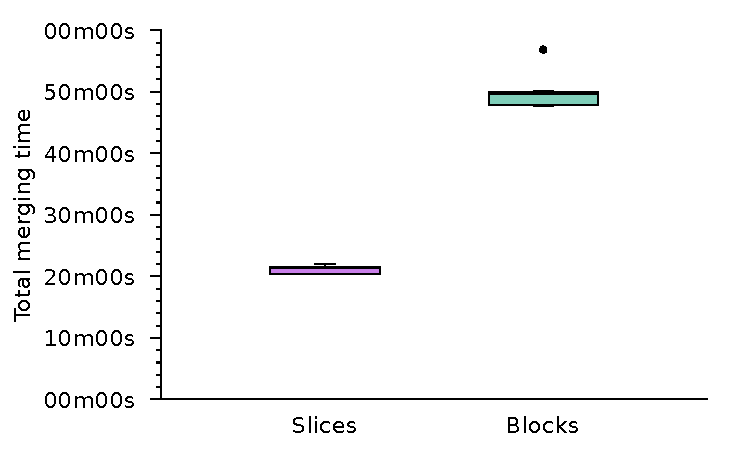
\includegraphics[width=0.45\columnwidth]{figures/blocks-slices/totalmergetimeSSD1.pdf}
  \hfill
  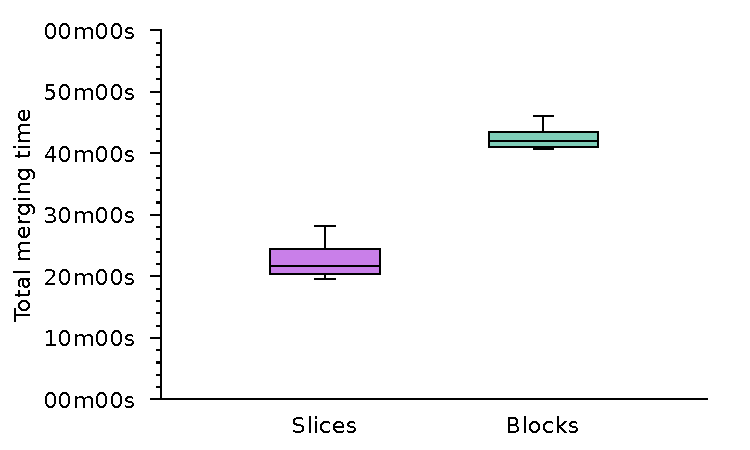
\includegraphics[width=0.45\columnwidth]{figures/blocks-slices/totalmergetimeHDD1.pdf}\\
  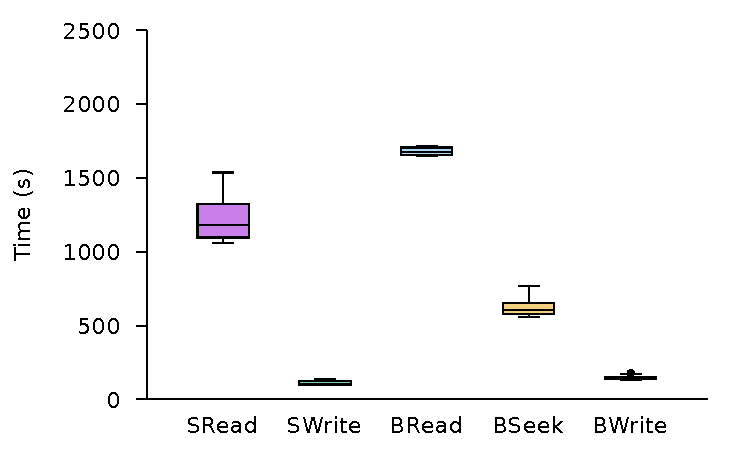
\includegraphics[width=0.45\columnwidth]{figures/blocks-slices/hddBreakDown1.pdf}
  \hfill
  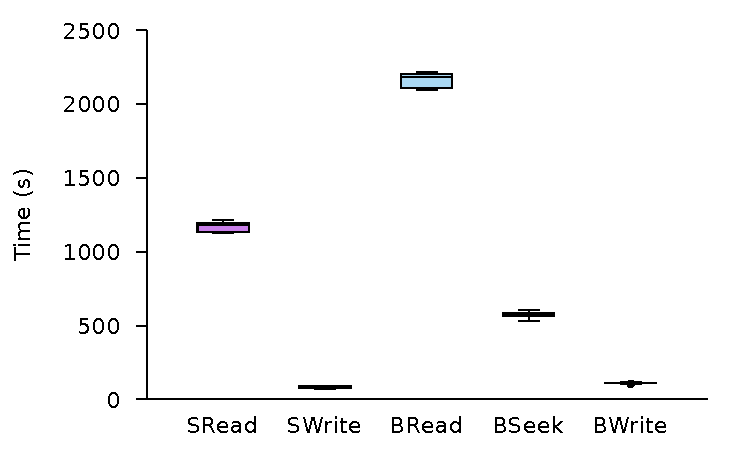
\includegraphics[width=0.45\columnwidth]{figures/blocks-slices/ssdBreakDown1.pdf}
  \caption{Merging time for Slices and Blocks. Left column: SSD. Right column: HDD. Top row: overall merging time. Bottom row: breakdown by read, write and seek time.}
  % Gnuplot file: scripts/blocks-slices/createboxplot.gnplt
\label{fig:slices-vs-blocks}
\end{figure}

\subsection{Buffered slices}

\subsection{Cluster reads}

\subsection{Multiple reads}

\begin{figure}[h]
  \centering
  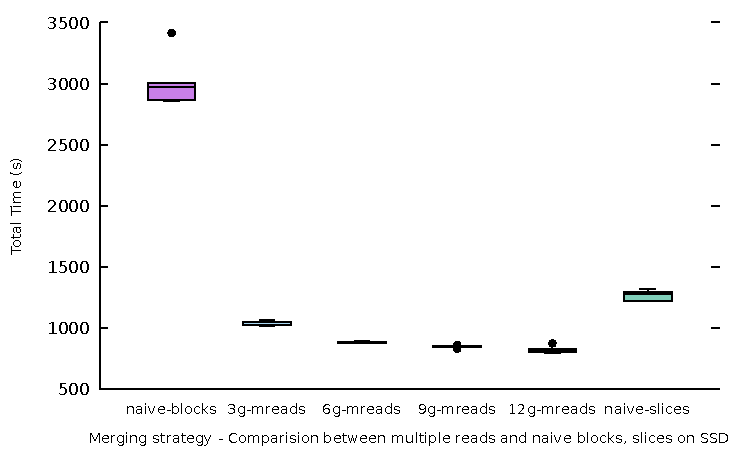
\includegraphics[width=0.45\columnwidth]{figures/benchmark-mreads/mreads-comparision-ssd.pdf}
  \hfill
  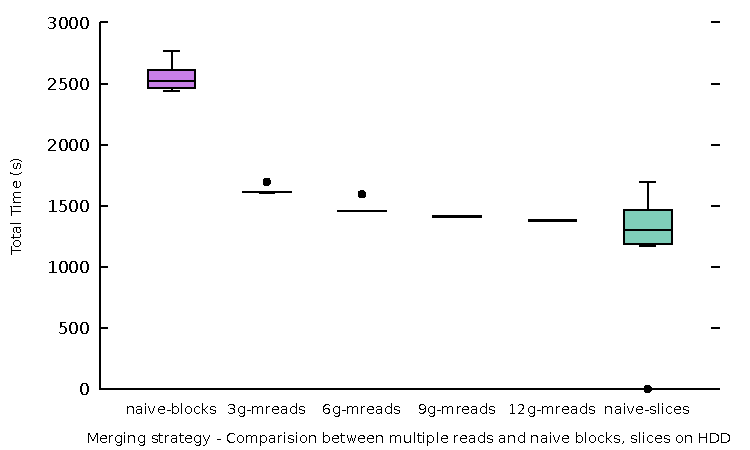
\includegraphics[width=0.45\columnwidth]{figures/benchmark-mreads/mreads-comparision-hdd.pdf}\\
  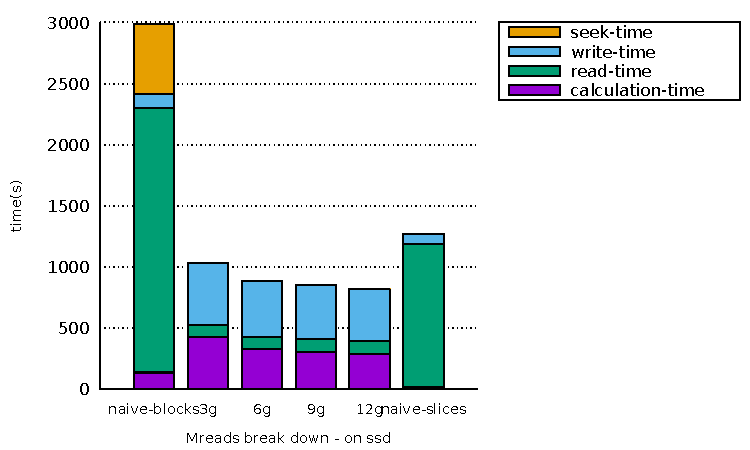
\includegraphics[width=0.45\columnwidth]{figures/benchmark-mreads/mreads-breakdown-ssd.pdf}
  \hfill
    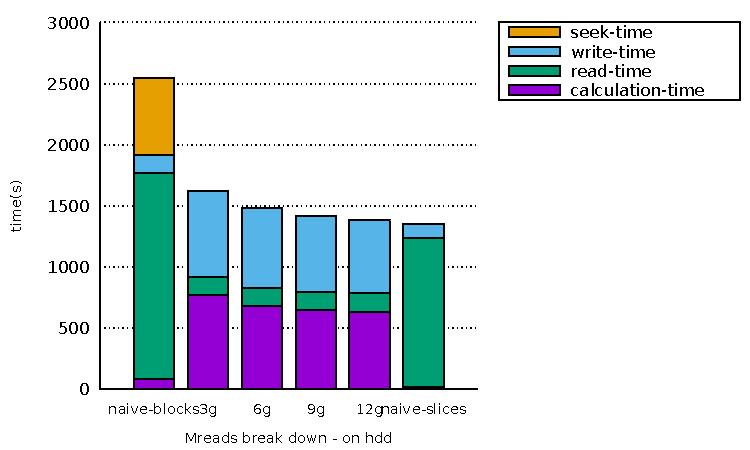
\includegraphics[width=0.45\columnwidth]{figures/benchmark-mreads/mreads-breakdown-hdd.pdf}
  \caption{Comparison between Multiple reads, blocks and slices. Left column: SSD. Right column: HDD. Top row: overall merging time. Bottom row: breakdown by read, write and seek time.}
  % Gnuplot file: scripts/blocks-slices/createboxplot.gnplt
\label{fig:multiple-reads}
\end{figure}

Results discussion:
\begin{itemize}
\item Comment on calculation time.
\item Write time is higher than read time because use nibabel for writing but not reading.
\item It seems that the merge time is quite stable w.r.t the amount of available memory. This is good news for multiple reads. 
\end{itemize}


\subsection{Cluster reads vs Multiple reads}

\subsubsection{Simulations}
After running a few simulations, we saw that the comparison between
Cluster reads and Multiple reads essentially depends on the three
Cluster reads configurations.  When Cluster reads merge incomplete
block rows (case 1), they are always outperformed by Multiple reads.
When Cluster reads merge complete block rows (case 2), the comparison
between Cluster reads and Multiple reads depends on the values of $D$
and $n$. Figure~\ref{fig:model-comparison} shows two situations where
Cluster reads and Multiple reads are alternatively better than each
other. When Cluster reads merge complete block slices (case 3),
Cluster reads and Multiple reads are equivalent.

\begin{figure}
  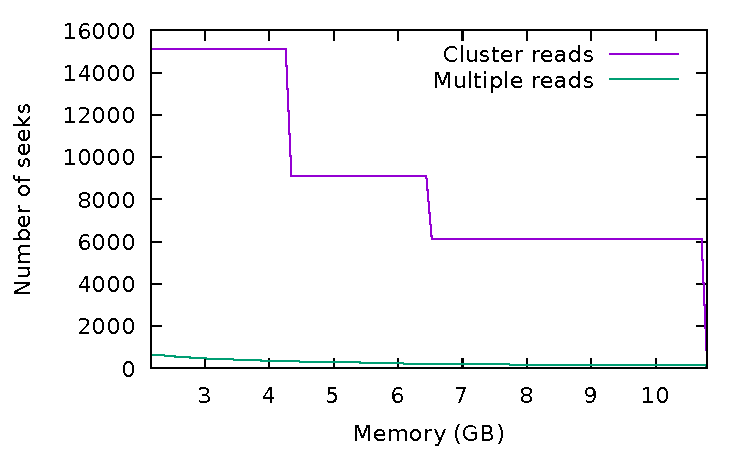
\includegraphics[width=0.45\columnwidth]{figures/model-big-brain.pdf}
  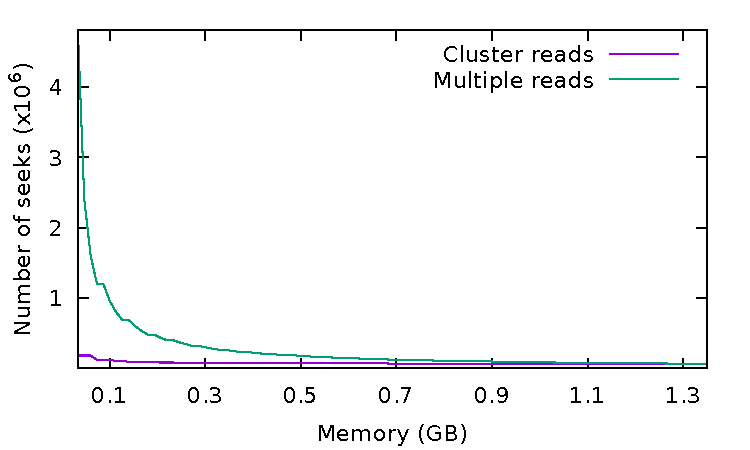
\includegraphics[width=0.45\columnwidth]{figures/model-big-brain-rescan.pdf}
  \caption{Number of seeks for Cluster reads vs Multiple reads when
    Cluster reads merge complete block rows (case 2), for D=3000 and
    b=2. Left: n=125; Right: n=64,000.}
  % Gnuplot file: scripts/model/model.gnplt
  \label{fig:model-comparison}
\end{figure}

\subsubsection{Experiments}

\subsection{Lossless Compression}

\subsection{Splitting}

\subsubsection{Multiple writes}
\begin{figure}[h]
  \centering
  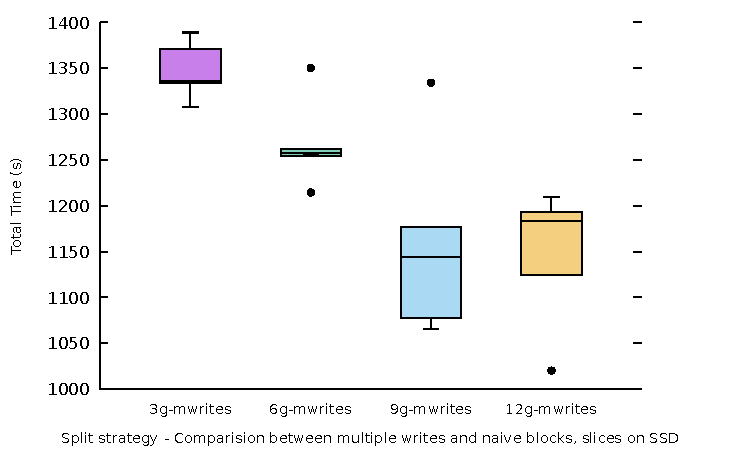
\includegraphics[width=0.45\columnwidth]{figures/benchmark-mwrites/mwrites-comparision-ssd.pdf}
  \hfill
  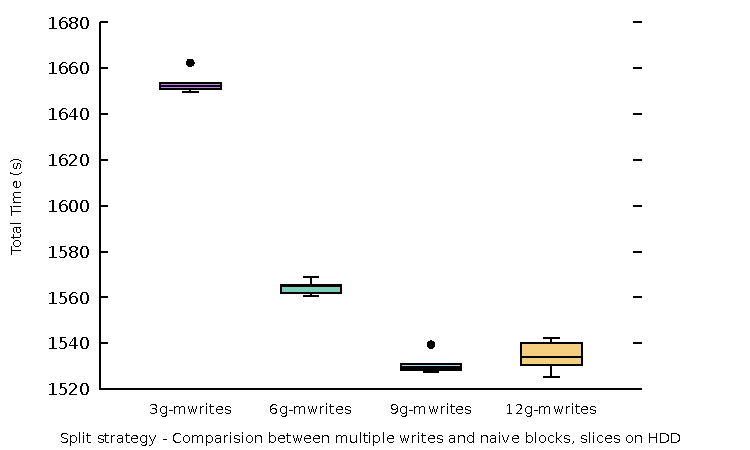
\includegraphics[width=0.45\columnwidth]{figures/benchmark-mwrites/mwrites-comparision-hdd.pdf}\\
  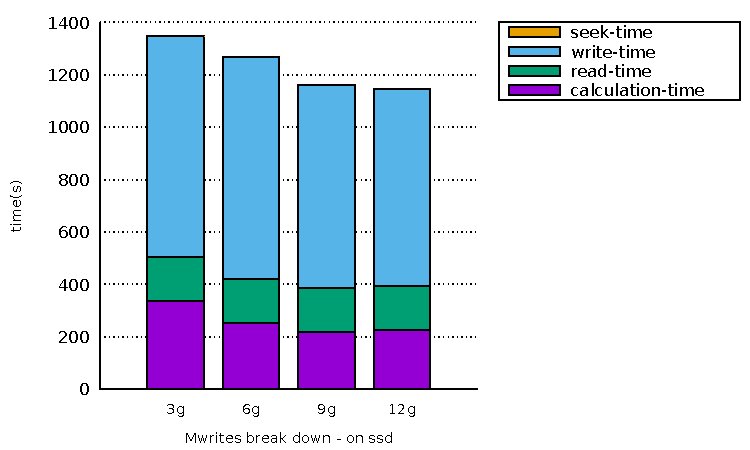
\includegraphics[width=0.45\columnwidth]{figures/benchmark-mwrites/mwrites-breakdown-ssd.pdf}
  \hfill
    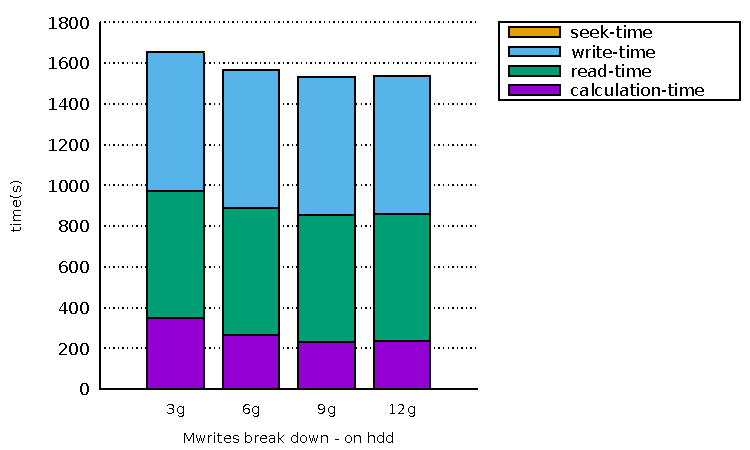
\includegraphics[width=0.45\columnwidth]{figures/benchmark-mwrites/mwrites-breakdown-hdd.pdf}
  \caption{Comparison between Multiple writes, blocks and slices. Left column: SSD. Right column: HDD. Top row: overall merging time. Bottom row: breakdown by read, write and seek time.}
  % Gnuplot file: scripts/blocks-slices/createboxplot.gnplt
\label{fig:multiple-writes}
\end{figure}


\newpage

\section{Discussion}
\label{sec:discussion}

What is the best algorithm (between 3 and 4), in which context. Did we
solve the seek problem or is there any issue remaining?

File formats:
\begin{itemize}
\item would MINC~\cite{vincent2016minc} support such algorithms? See on-going email discussion
with P. Bellec.
\item some formats optimize the storage for particular split shapes. See
  ndstore~\cite{burns2013open}. Such formats would behave equally
  poorly with chunks that do not comply to this geometry. Our
  algorithms would work equally well with such formats.
\end{itemize}

The performance model might be dependent on the particular
infrastructure (disks, OS and filesystem) used in the experiments. In
particular, caching might behave differently in a different setup.

Reconstructing (therefore splitting) a complete 3D image may not
always be necessary. Re-splitting, for instance, could be done from
existing chunks.

\section{Conclusion}

Future work:
- obliques
- parallel algorithms
- re-splitting
- model

% Ideas for the future: measure the actual amount of consumed memory.

\section*{Acknowledgment}

(If not added as co-authors): Greg Kiar, Pierre Bellec.

\bibliographystyle{IEEEtran}
\bibliography{IEEEabrv,biblio.bib}

\end{document}
